% ===========================================================================
% Presentación resumen del TFM — MADI, Tecnun
%
% Formato 16:9. No usa beamer (no está instalado en este equipo y además su
% maquetación por defecto es reconocible); se compone sobre `article` con una
% geometría de diapositiva y macros propias.
%
% Compilar:  bash compilar.sh    (desde presentacion/)
% ===========================================================================
\documentclass[12pt]{article}

\usepackage[utf8]{inputenc}
\usepackage[T1]{fontenc}
\usepackage[spanish,es-noshorthands]{babel}
\usepackage[sfdefault]{FiraSans}
\usepackage{textcomp}
\usepackage{microtype}

\usepackage[papersize={25.4cm,14.29cm},
            left=1.7cm,right=1.7cm,top=1.0cm,bottom=0.8cm,
            footskip=0.55cm]{geometry}

\usepackage{xcolor}
\usepackage{graphicx}
\usepackage{booktabs}
\usepackage{array}
\usepackage{tikz}
\usetikzlibrary{arrows.meta,positioning,calc,fit,backgrounds}
\usepackage{fancyhdr}
\usepackage[hidelinks]{hyperref}

% --- Paleta -----------------------------------------------------------------
% Los mismos colores que las figuras de la memoria: el deck y el documento
% deben leerse como una sola pieza.
\definecolor{tinta}{HTML}{0B0B0B}
\definecolor{grisTexto}{HTML}{52514E}
\definecolor{azul}{HTML}{2A78D6}
\definecolor{naranja}{HTML}{EB6834}
\definecolor{aqua}{HTML}{1BAF7A}
\definecolor{regla}{HTML}{D5D4CF}
\definecolor{suave}{HTML}{F5F4F1}

\graphicspath{{../memoria/figuras/}}

% --- Estructura de la diapositiva -------------------------------------------
\setlength{\parindent}{0pt}
\setlength{\parskip}{0pt}
\renewcommand{\arraystretch}{1.15}

\newcommand{\seccionActual}{}
\pagestyle{fancy}
\fancyhf{}
\renewcommand{\headrulewidth}{0pt}
\renewcommand{\footrulewidth}{0pt}
\fancyfoot[L]{\footnotesize\color{grisTexto}\seccionActual}
\fancyfoot[R]{\footnotesize\color{grisTexto}\thepage}

% \diapo{sección}{título} — abre una diapositiva.
%
% El \typeout deja en presentacion.log la altura consumida por la diapositiva
% que se acaba de cerrar. Si `usado` supera a `de`, esa diapositiva se parte en
% dos páginas (el contenido baja entero y el título se queda solo). Es la forma
% rápida de saber CUÁNTO hay que recortar en lugar de ir probando:
%     grep -a MEDIDA presentacion.log
\newcommand{\diapo}[2]{%
  \typeout{MEDIDA pagina \thepage: usado=\the\pagetotal\space de \the\pagegoal}%
  \clearpage
  \renewcommand{\seccionActual}{#1}%
  {\color{azul}\rule{2.4cm}{2pt}}\par\vspace{0.38em}
  {\fontsize{18}{21}\selectfont\bfseries\color{tinta}#2}\par\vspace{0.3em}
  {\color{regla}\rule{\linewidth}{0.4pt}}\par\vspace{0.7em}
}

% Bloque de texto con filete de acento a la izquierda
% \bloque{color}{titulillo}{texto}
% Sin entorno `list`: éste añadía \partopsep/\parsep implícitos que
% descuadraban la altura de la diapositiva. Aquí el espaciado es explícito.
% El bloque se compone primero en una caja para poder medirlo y dibujar el
% filete de acento con la altura exacta del bloque completo.
\newsavebox{\cajaBloque}
\newcommand{\bloque}[3]{%
  \par\noindent
  \begin{lrbox}{\cajaBloque}%
    \begin{minipage}[t]{\dimexpr\linewidth-2pt-0.62em\relax}
      \raggedright
      {\fontsize{11.5}{14}\selectfont\bfseries\color{tinta}#2\par}\vspace{0.12em}
      {\fontsize{10.5}{13.2}\selectfont\color{grisTexto}#3\par}
    \end{minipage}%
  \end{lrbox}%
  {\color{#1}\rule[-\dp\cajaBloque]{2pt}%
    {\dimexpr\ht\cajaBloque+\dp\cajaBloque\relax}}%
  \hspace{0.62em}\usebox{\cajaBloque}\par\vspace{0.55em}%
}

% Cifra destacada: \cifra{color}{valor}{descripción}
% En columnas estrechas la justificación abre huecos y fuerza guiones; todo el
% texto de cuerpo va en bandera a la derecha.
\newcommand{\cifra}[3]{%
  {\fontsize{23}{25}\selectfont\bfseries\color{#1}#2}\par\vspace{0.1em}
  {\raggedright\fontsize{9.5}{12}\selectfont\color{grisTexto}#3\par}\vspace{0.65em}
}

\newcommand{\nota}[1]{%
  \vspace{0.2em}{\raggedright\fontsize{9}{11.5}\selectfont\color{grisTexto}#1\par}}

\newcommand{\cuerpo}[1]{%
  {\raggedright\fontsize{11}{14.3}\selectfont\color{grisTexto}#1\par}}

\newcommand{\pie}[1]{%
  \vspace{0.35em}{\raggedright\fontsize{8.5}{11}\selectfont\color{grisTexto}#1\par}}

% Ítem con viñeta de guion, sobrio
\newenvironment{puntos}[1][11.5]{%
  \begin{list}{\textcolor{azul}{\rule[0.28em]{0.5em}{1pt}}}%
    {\leftmargin=1.35em\itemsep=0.45em\parsep=0pt\topsep=0.2em
     \fontsize{#1}{15}\selectfont\color{grisTexto}}}%
  {\end{list}}

\begin{document}

% ===========================================================================
% 1 — PORTADA
% ===========================================================================
\thispagestyle{empty}
\vspace*{0.7cm}
{\color{azul}\rule{4.2cm}{3pt}}\par\vspace{1.5em}

{\fontsize{11}{14}\selectfont\color{grisTexto}%
Tecnun --- Escuela de Ingeniería, Universidad de Navarra\par
Máster Universitario en Análisis de Datos en Ingeniería (MADI)\par}

\vspace{1.5em}

{\fontsize{25}{31}\selectfont\bfseries\color{tinta}%
Aprendizaje federado para la previsión\\ de demanda en \emph{retail}\par}

\vspace{0.5em}
{\fontsize{14}{18}\selectfont\color{grisTexto}%
Evaluación frente a modelos locales, centralizados y convencionales\par}

\vfill

\begin{minipage}[b]{0.5\linewidth}
  {\fontsize{13}{16}\selectfont\bfseries\color{tinta}Alessandro Flammia\par}
  \vspace{0.25em}
  {\fontsize{11}{14}\selectfont\color{grisTexto}Tutora: Idoia Ochoa\par}
\end{minipage}%
\begin{minipage}[b]{0.5\linewidth}
  \raggedleft
  {\fontsize{11}{14}\selectfont\color{grisTexto}%
  Resumen de la memoria del Trabajo Fin de Máster\par
  Septiembre de 2026\par}
\end{minipage}

\vspace{0.6cm}

% ===========================================================================
% 2 — CONTENIDO
% ===========================================================================
\diapo{Contenido}{Qué contiene esta presentación}

\begin{minipage}[t]{0.5\linewidth}
\bloque{azul}{1. El problema}{Por qué los datos que mejorarían la previsión
  están en manos de quien no puede compartirlos.}
\bloque{azul}{2. El enfoque y las preguntas}{Qué es el aprendizaje federado y
  qué se pregunta exactamente este trabajo.}
\bloque{azul}{3. Datos y método}{Un histórico real de 54 tiendas, cinco
  condiciones experimentales y un único protocolo de evaluación.}
\bloque{azul}{4. Resultados}{Qué funcionó, qué no, y qué dice el contraste
  estadístico sobre cada diferencia.}
\end{minipage}\hfill
\begin{minipage}[t]{0.44\linewidth}
\bloque{aqua}{5. Del simulador a la nube}{Verificación del esquema sobre tres
  máquinas independientes con aislamiento real de datos.}
\bloque{aqua}{6. Valor de negocio}{Cuánto vale colaborar, para quién, y dónde
  la cifra agregada esconde matices.}
\bloque{aqua}{7. Conclusiones}{Respuesta a las cinco preguntas de
  investigación y líneas abiertas.}

\vspace{0.6em}
\nota{Todas las cifras de esta presentación proceden de los resultados
  documentados en la memoria y son trazables a los ficheros de resultados del
  repositorio.}
\end{minipage}

% ===========================================================================
% 3 — EL PROBLEMA
% ===========================================================================
\diapo{1. El problema}{Los datos que harían falta no se pueden compartir}

\begin{minipage}[t]{0.5\linewidth}
\vspace{0pt}
\bloque{tinta}{La previsión mejora con más datos}{Un operador con más tiendas y
  más historial dispone de más señal para estimar la demanda: más patrones
  estacionales, más respuestas a promoción, más casos de cada familia de
  producto.}

\bloque{naranja}{Pero los datos están repartidos entre competidores}{Los
  operadores que más se beneficiarían de un modelo conjunto compiten entre sí.
  Ceder el histórico de ventas no es viable ni comercial ni legalmente.}

\bloque{tinta}{Resultado: cada uno entrena en solitario}{Con una fracción de los
  datos que realmente existen sobre el mismo problema.}

\vspace{0.3em}
\cuerpo{\bfseries\color{tinta}¿Se puede entrenar un modelo conjunto sin que
  nadie ceda sus datos?}
\end{minipage}\hfill
\begin{minipage}[t]{0.45\linewidth}
\vspace{0.6cm}
\centering
\begin{tikzpicture}[
    op/.style={draw=regla,fill=suave,rounded corners=2pt,minimum width=2.5cm,
               minimum height=1.0cm,align=center,font=\footnotesize\color{tinta}},
    >={Stealth[round]}]
  \node[op] (a) at (-3.1,0) {\textbf{Operador A}\\{\scriptsize sus datos}};
  \node[op] (b) at (0,0)    {\textbf{Operador B}\\{\scriptsize sus datos}};
  \node[op] (c) at (3.1,0)  {\textbf{Operador C}\\{\scriptsize sus datos}};

  \node[draw=regla,rounded corners=2pt,minimum width=5.0cm,minimum height=1.0cm,
        align=center,font=\footnotesize\color{tinta}] (m) at (0,-2.9)
        {\textbf{Modelo conjunto}\\{\scriptsize más datos, mejor previsión}};

  \foreach \n in {a,b,c}{
    \draw[->,grisTexto,line width=0.9pt,opacity=0.55] (\n) -- (m);
  }
  \foreach \x in {-1.62,0,1.62}{
    \node[fill=white,inner sep=1pt] at (\x,-1.45)
      {\textcolor{naranja}{\bfseries\Large $\times$}};
  }

  \node[font=\scriptsize\color{naranja},align=center] at (0,-3.85)
    {la cesión de datos crudos es inviable};
\end{tikzpicture}
\end{minipage}

% ===========================================================================
% 4 — EL ENFOQUE
% ===========================================================================
\diapo{2. El enfoque}{Aprendizaje federado: circulan los parámetros, no los datos}

\begin{minipage}[t]{0.46\linewidth}
\vspace{0pt}
\cuerpo{En lugar de reunir los datos en un sitio, cada participante entrena
  \textbf{con los suyos} y envía únicamente los \textbf{pesos} del modelo. Un
  coordinador los promedia y devuelve el modelo global. Se repite por rondas.}

\vspace{0.9em}
\bloque{azul}{Los datos no salen nunca del silo}{El coordinador no custodia
  datos: solo maneja parámetros y un conjunto de validación de referencia.}

\bloque{azul}{Participan los silos, no las tiendas}{Escenario \emph{cross-silo}:
  tres participantes, cada uno con sus propias tiendas centralizadas
  internamente, que es legítimo porque son del mismo operador.}

\pie{Advertencia recogida en la memoria: los parámetros intercambiados pueden
  seguir constituyendo datos personales (AEPD y EDPS, 2025). El esquema reduce
  la exposición, pero por sí solo no anonimiza.}
\end{minipage}\hfill
\begin{minipage}[t]{0.5\linewidth}
\vspace{0.15cm}
\centering
\begin{tikzpicture}[
    nodo/.style={draw=regla,rounded corners=2pt,minimum width=2.4cm,
                 minimum height=0.95cm,align=center,
                 font=\footnotesize\color{tinta}},
    >={Stealth[round]}]
  \node[nodo,fill=suave] (srv) {\textbf{Coordinador}\\{\scriptsize promedia los parámetros}};
  \node[nodo,below left=1.75cm and 1.25cm of srv] (s1)
    {\textbf{Silo Grande}\\{\scriptsize 9 tiendas}};
  \node[nodo,below=1.75cm of srv] (s2)
    {\textbf{Silo Mediano}\\{\scriptsize 26 tiendas}};
  \node[nodo,below right=1.75cm and 1.25cm of srv] (s3)
    {\textbf{Silo Pequeño}\\{\scriptsize 19 tiendas}};

  \foreach \s in {s1,s2,s3}{
    \draw[->,azul,line width=0.8pt] (srv) to[bend right=13] (\s);
    \draw[->,grisTexto,dashed,line width=0.6pt] (\s) to[bend right=13] (srv);
  }
  % Leyenda debajo del conjunto: a la derecha del coordinador desbordaba
  % el ancho de la columna.
  \node[font=\scriptsize\color{grisTexto},align=center,below=0.3cm of s2]
    {los datos nunca salen del silo};
  \node[font=\scriptsize,align=center,below=0.95cm of s2]
    {\textcolor{azul}{\textbf{---}}~{\color{grisTexto}modelo global}\qquad
     \textcolor{grisTexto}{\textbf{-\,-}}~{\color{grisTexto}parámetros locales}};
\end{tikzpicture}
\end{minipage}

% ===========================================================================
% 5 — PREGUNTAS DE INVESTIGACIÓN
% ===========================================================================
\diapo{2. El enfoque}{Las cinco preguntas de investigación}

\begin{minipage}[t]{0.56\linewidth}
\vspace{0pt}
\bloque{azul}{RQ1 — técnica}{¿Predice el federado mejor que el modelo local de
  cada tienda y se aproxima al centralizado, sin compartir datos crudos?
  Incluye la personalización posterior como variante.}
\bloque{azul}{RQ2 — técnica}{¿Supera a los métodos convencionales: baselines
  ingenuos, suavizado exponencial y árboles potenciados por gradiente?}
\bloque{aqua}{RQ3 — negocio}{¿Qué valor económico genera la mejora de precisión
  atribuible a la colaboración?}
\bloque{aqua}{RQ4 — negocio}{¿Por qué un esquema federado y no un \emph{data
  clean room}?}
\bloque{grisTexto}{RQ5 — ampliación}{¿Qué coste en precisión tendría añadir
  privacidad diferencial? \emph{No se aborda; queda como línea futura.}}
\end{minipage}\hfill
\begin{minipage}[t]{0.38\linewidth}
\vspace{0.4cm}
\colorbox{suave}{%
\begin{minipage}{\dimexpr\linewidth-1.6em}
\vspace{0.7em}\raggedright
{\fontsize{12.5}{15}\selectfont\bfseries\color{tinta}Una formulación neutra\par}
\vspace{0.5em}
{\fontsize{11}{14.5}\selectfont\color{grisTexto}%
El trabajo no parte de la hipótesis de que el aprendizaje federado sea
superior, sino de la pregunta de si lo es.\par\vspace{0.5em}
Admite como resultado válido que \textbf{no} lo sea --- y, como se verá, esa es
en parte la respuesta.\par}
\vspace{0.9em}
\end{minipage}}
\end{minipage}

% ===========================================================================
% 6 — DATOS
% ===========================================================================
\diapo{3. Datos y método}{Un histórico real, dividido en silos heterogéneos}

\begin{minipage}[t]{0.44\linewidth}
\vspace{0pt}
\bloque{tinta}{Corporación Favorita (Ecuador), datos abiertos}{Ventas de
  \textbf{54 tiendas} y \textbf{33 familias} entre 2013 y 2017, con festivos,
  precio del petróleo y promociones.}

\bloque{tinta}{Granularidad: tienda × familia × semana}{\textbf{1.782 series} y
  322.245 filas. Es la granularidad de la reposición agregada y evita la
  intermitencia del nivel diario por referencia.}

\bloque{azul}{Silos por formato de tienda}{Grande (9), Mediano (26) y Pequeño
  (19). La heterogeneidad está sobre todo en la \emph{escala} de venta ---
  factores de 2 a 3 veces --- y en la intensidad promocional.}

\bloque{tinta}{Partición temporal estricta}{220 semanas de entrenamiento, 8 de
  validación y 8 de prueba, en orden cronológico.}
\end{minipage}\hfill
\begin{minipage}[t]{0.52\linewidth}
\vspace{0pt}
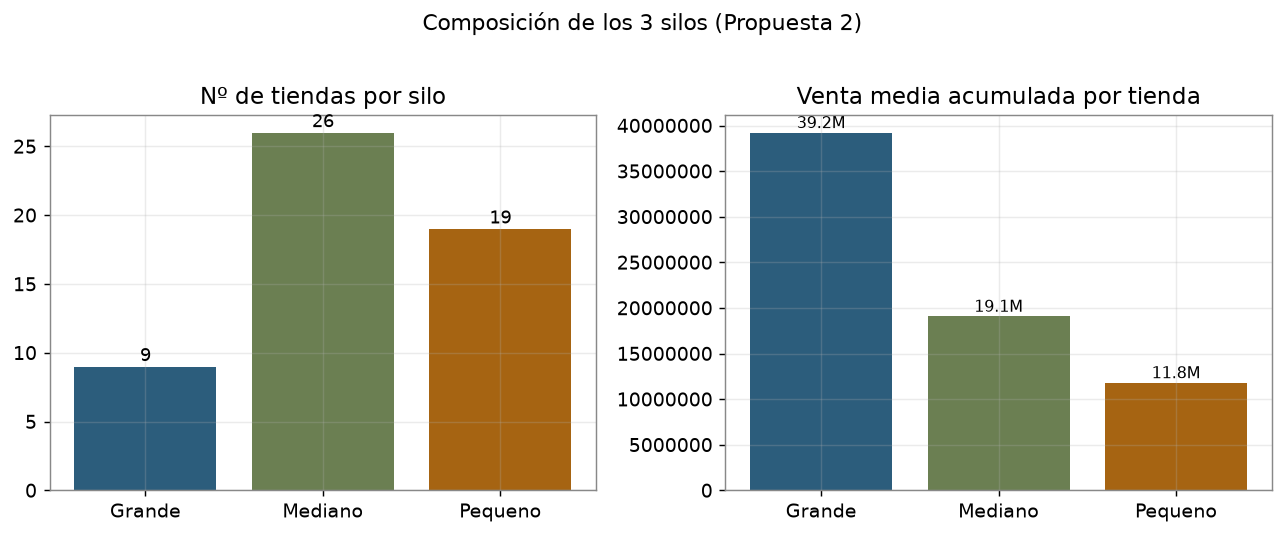
\includegraphics[width=\linewidth]{datos_composicion_silos.png}
\pie{\textbf{Limitación declarada:} los silos son formatos de tienda de una
  misma cadena, no operadores competidores reales. Es la metodología estándar
  del campo ante la ausencia de datos públicos entre cadenas, y se declara
  explícitamente como limitación del estudio.}
\pie{\textbf{Nota metodológica:} se detectó y corrigió un desalineamiento
  silencioso de los retardos causado por el hueco del 25 de diciembre, que
  afectaba a 1.749 de las 1.782 series.}
\end{minipage}

% ===========================================================================
% 7 — DISEÑO EXPERIMENTAL
% ===========================================================================
\diapo{3. Datos y método}{Cinco condiciones, un mismo modelo, un mismo protocolo}

\begin{minipage}[t]{0.53\linewidth}
\vspace{0pt}
% Columnas `l` (sin ajuste de línea): cada condición ocupa exactamente una
% línea y las descripciones quedan alineadas.
{\fontsize{10.5}{14.5}\selectfont
\begin{tabular}{@{}l@{\hspace{0.9em}}l@{}}
{\color{tinta}\textbf{A} — Local} &
  {\color{grisTexto}un modelo por tienda, sin colaboración} \\
{\color{tinta}\textbf{B} — Centralizado por silo} &
  {\color{grisTexto}un modelo por formato de tienda} \\
{\color{tinta}\textbf{C} — Centralizado global} &
  {\color{grisTexto}un modelo con los tres silos juntos} \\
{\color{azul}\textbf{D} — Federado} &
  {\color{grisTexto}FedAvg entre los silos (y FedProx)} \\
{\color{azul}\textbf{E} — Federado + person.} &
  {\color{grisTexto}ajuste fino por tienda sobre D} \\
\end{tabular}\par}

\vspace{0.9em}
\bloque{tinta}{Referencias externas}{Persistencia, estacional de 52 semanas,
  media móvil de 4 semanas, ETS/Holt-Winters y un \textbf{LightGBM global},
  como exigencia máxima no federada.}

\bloque{tinta}{Métrica y contraste}{WMAPE por serie, agregado por la mediana.
  Test de \textbf{Wilcoxon pareado} con corrección de
  \textbf{Holm-Bonferroni}.}
\end{minipage}\hfill
\begin{minipage}[t]{0.42\linewidth}
\vspace{0.3cm}
\centering
{\fontsize{10.5}{13}\selectfont\bfseries\color{tinta}%
El modelo, común a las cinco condiciones\par}
\vspace{0.7em}
\begin{tikzpicture}[
    caja/.style={draw=regla,rounded corners=2pt,minimum height=0.72cm,
                 align=center,font=\scriptsize\color{tinta}},
    >={Stealth[round]},node distance=0.4cm]
  \node[caja,minimum width=2.5cm,fill=suave] (cont) {17 variables continuas};
  \node[caja,minimum width=2.5cm,below=of cont,fill=suave] (fam)
    {\emph{embedding} familia\\33 $\rightarrow$ 8};
  \node[caja,minimum width=2.5cm,below=of fam,fill=suave] (tie)
    {\emph{embedding} tienda\\54 $\rightarrow$ 8};
  \node[caja,right=0.85cm of fam,minimum width=1.0cm] (concat) {conc.\\33};
  \node[caja,right=0.35cm of concat,minimum width=1.0cm] (h1) {Densa\\64};
  \node[caja,right=0.3cm of h1,minimum width=1.0cm] (h2) {Densa\\32};
  \node[caja,right=0.3cm of h2,minimum width=1.0cm,draw=azul] (out) {Salida\\1};
  \draw[->,grisTexto] (cont.east) -- (concat.west);
  \draw[->,grisTexto] (fam.east) -- (concat.west);
  \draw[->,grisTexto] (tie.east) -- (concat.west);
  \draw[->,grisTexto] (concat) -- (h1);
  \draw[->,grisTexto] (h1) -- (h2);
  \draw[->,grisTexto] (h2) -- (out);
\end{tikzpicture}
\vspace{0.5em}
\pie{Perceptrón multicapa con \emph{embeddings} de entidad: \textbf{4.985
  parámetros}. El tamaño reducido es deliberado --- en federado el coste de
  comunicación es proporcional a los parámetros que se intercambian en cada
  ronda.}
\end{minipage}

% ===========================================================================
% 8 — RESULTADO 1
% ===========================================================================
\diapo{4. Resultados}{Dos resultados que contradicen la hipótesis de partida}

\begin{minipage}[t]{0.47\linewidth}
\vspace{0pt}
{\fontsize{9}{11.5}\selectfont\color{grisTexto}%
WMAPE en prueba (mediana de las series)\par}
\vspace{0.35em}
{\fontsize{10.5}{14}\selectfont
\begin{tabular}{@{}l@{\hspace{1.2em}}r@{}}
{\color{tinta}C — Centralizado global}   & {\color{tinta}0,1736} \\
{\color{tinta}B — Centralizado por silo} & {\color{tinta}0,1676} \\
{\color{tinta}A — Local}                 & {\color{tinta}0,1476} \\
{\color{azul}D — Federado}               & {\color{azul}0,1507} \\
\textbf{\color{azul}E — Federado + person.} & \textbf{\color{azul}0,1379} \\
\end{tabular}\par}

\vspace{0.9em}
\bloque{naranja}{Centralizar empeora, de forma monótona}{El modelo global (C)
  dispone de unas 54 veces más datos que un modelo local y es \textbf{el peor de
  los cinco}. No es falta de entrenamiento: más paciencia solo produce
  sobreajuste.}

\bloque{azul}{Federar sin personalizar no compensa}{D (0,1507) \textbf{no
  alcanza} al modelo local A (0,1476). Es el ajuste fino por tienda el que
  convierte al federado en la mejor de las cinco condiciones.}
\end{minipage}\hfill
\begin{minipage}[t]{0.49\linewidth}
\vspace{0pt}
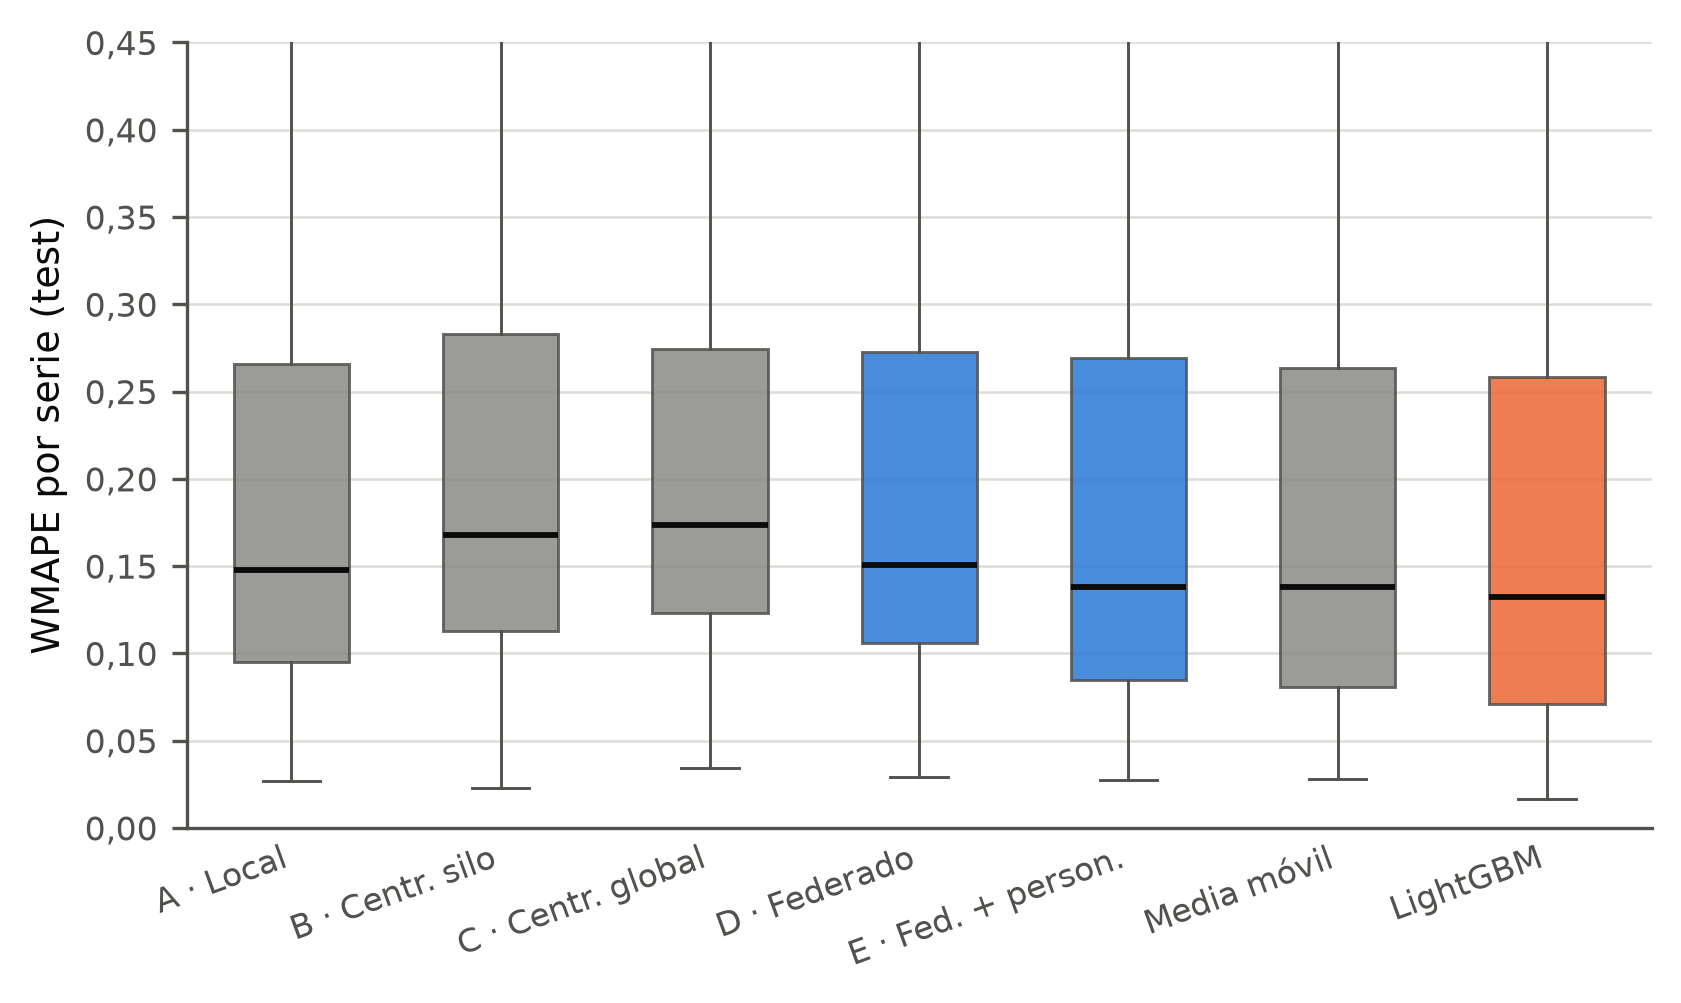
\includegraphics[width=\linewidth]{resultados_distribucion_por_serie.png}
\pie{La diferencia entre condiciones es pequeña frente a la variabilidad entre
  series: las medianas ordenan bien los métodos, pero conviven con una
  dispersión considerable. De ahí la necesidad del contraste pareado.}
\end{minipage}

% ===========================================================================
% 9 — RESULTADO 2
% ===========================================================================
\diapo{4. Resultados}{Frente a los métodos convencionales: el federado no gana}

\begin{minipage}[t]{0.55\linewidth}
\vspace{0pt}
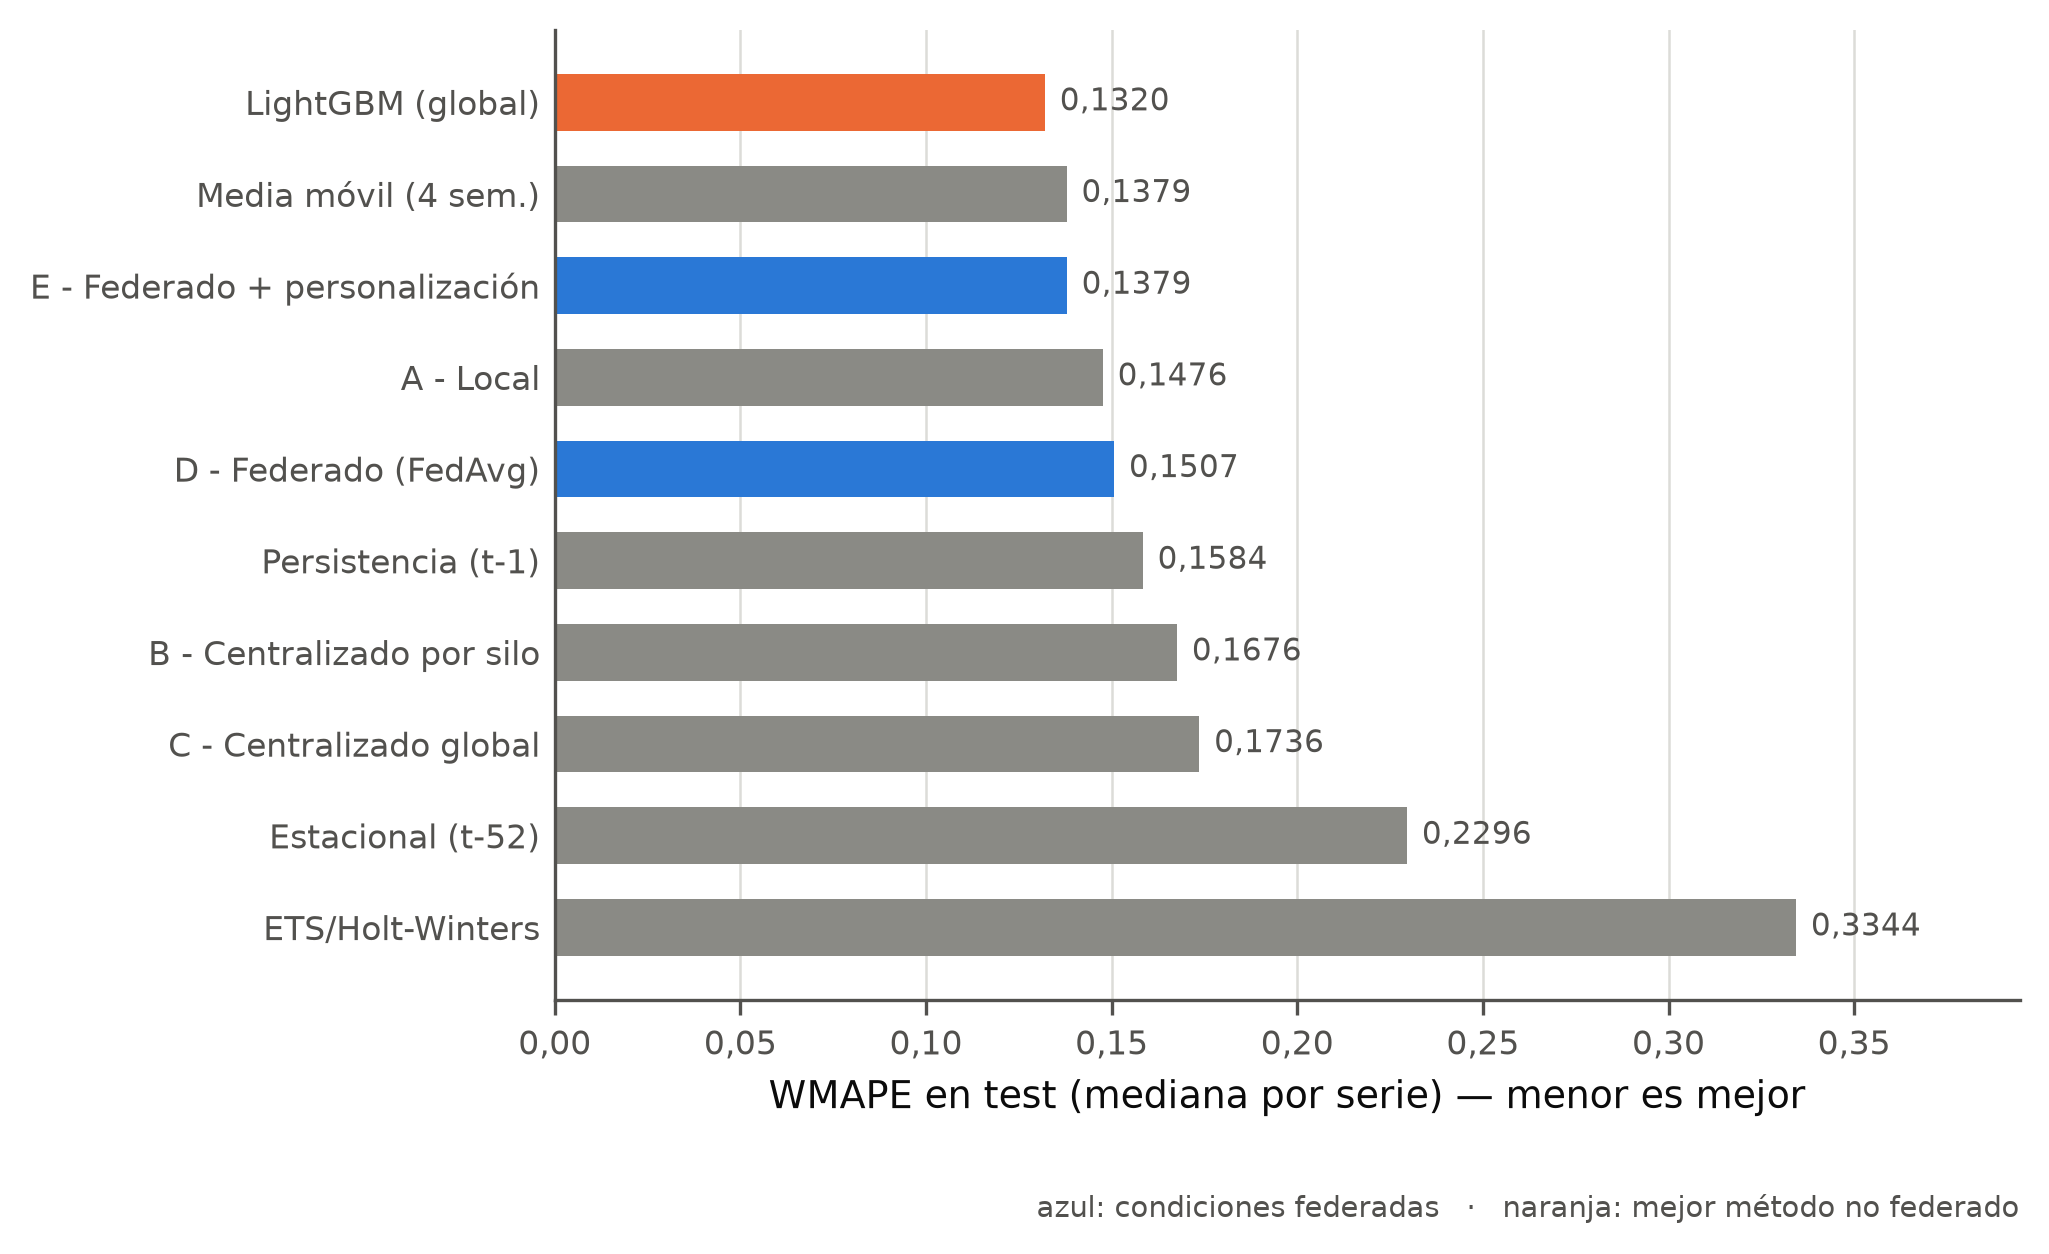
\includegraphics[width=\linewidth]{resultados_comparativa_metodos.png}
\end{minipage}\hfill
\begin{minipage}[t]{0.41\linewidth}
\vspace{0pt}
\bloque{naranja}{El mejor método del estudio no es federado}{Un
  \textbf{LightGBM global} sobre los datos agrupados obtiene 0,1320 frente a
  los 0,1379 de la mejor condición federada.}

\bloque{tinta}{La media móvil de 4 semanas iguala en mediana}{El más simple de
  los métodos alcanza también 0,1379. El contraste pareado matiza este aparente
  empate.}

\colorbox{suave}{%
\begin{minipage}{\dimexpr\linewidth-1.4em}
\vspace{0.55em}
{\fontsize{10}{13}\selectfont\color{grisTexto}%
\textbf{\color{tinta}¿Y si el federado solo estaba mal ajustado?}
Se hizo búsqueda de hiperparámetros: mejoró D un 7\,\%
(0,1507 $\rightarrow$ 0,1402), pero \textbf{no se trasladó} a E. La conclusión
no cambia.\par}
\vspace{0.55em}
\end{minipage}}

\vspace{0.7em}
{\fontsize{10.5}{13.5}\selectfont\bfseries\color{tinta}El valor del federado no
  está en la precisión absoluta, sino en alcanzar un rendimiento comparable
  \emph{sin centralizar los datos} --- que es justo lo que los métodos que lo
  superan sí exigen.\par}
\end{minipage}

% ===========================================================================
% 10 — CONTRASTE ESTADÍSTICO
% ===========================================================================
\diapo{4. Resultados}{Ninguna de estas diferencias es ruido}

\begin{minipage}[t]{0.53\linewidth}
\vspace{0pt}
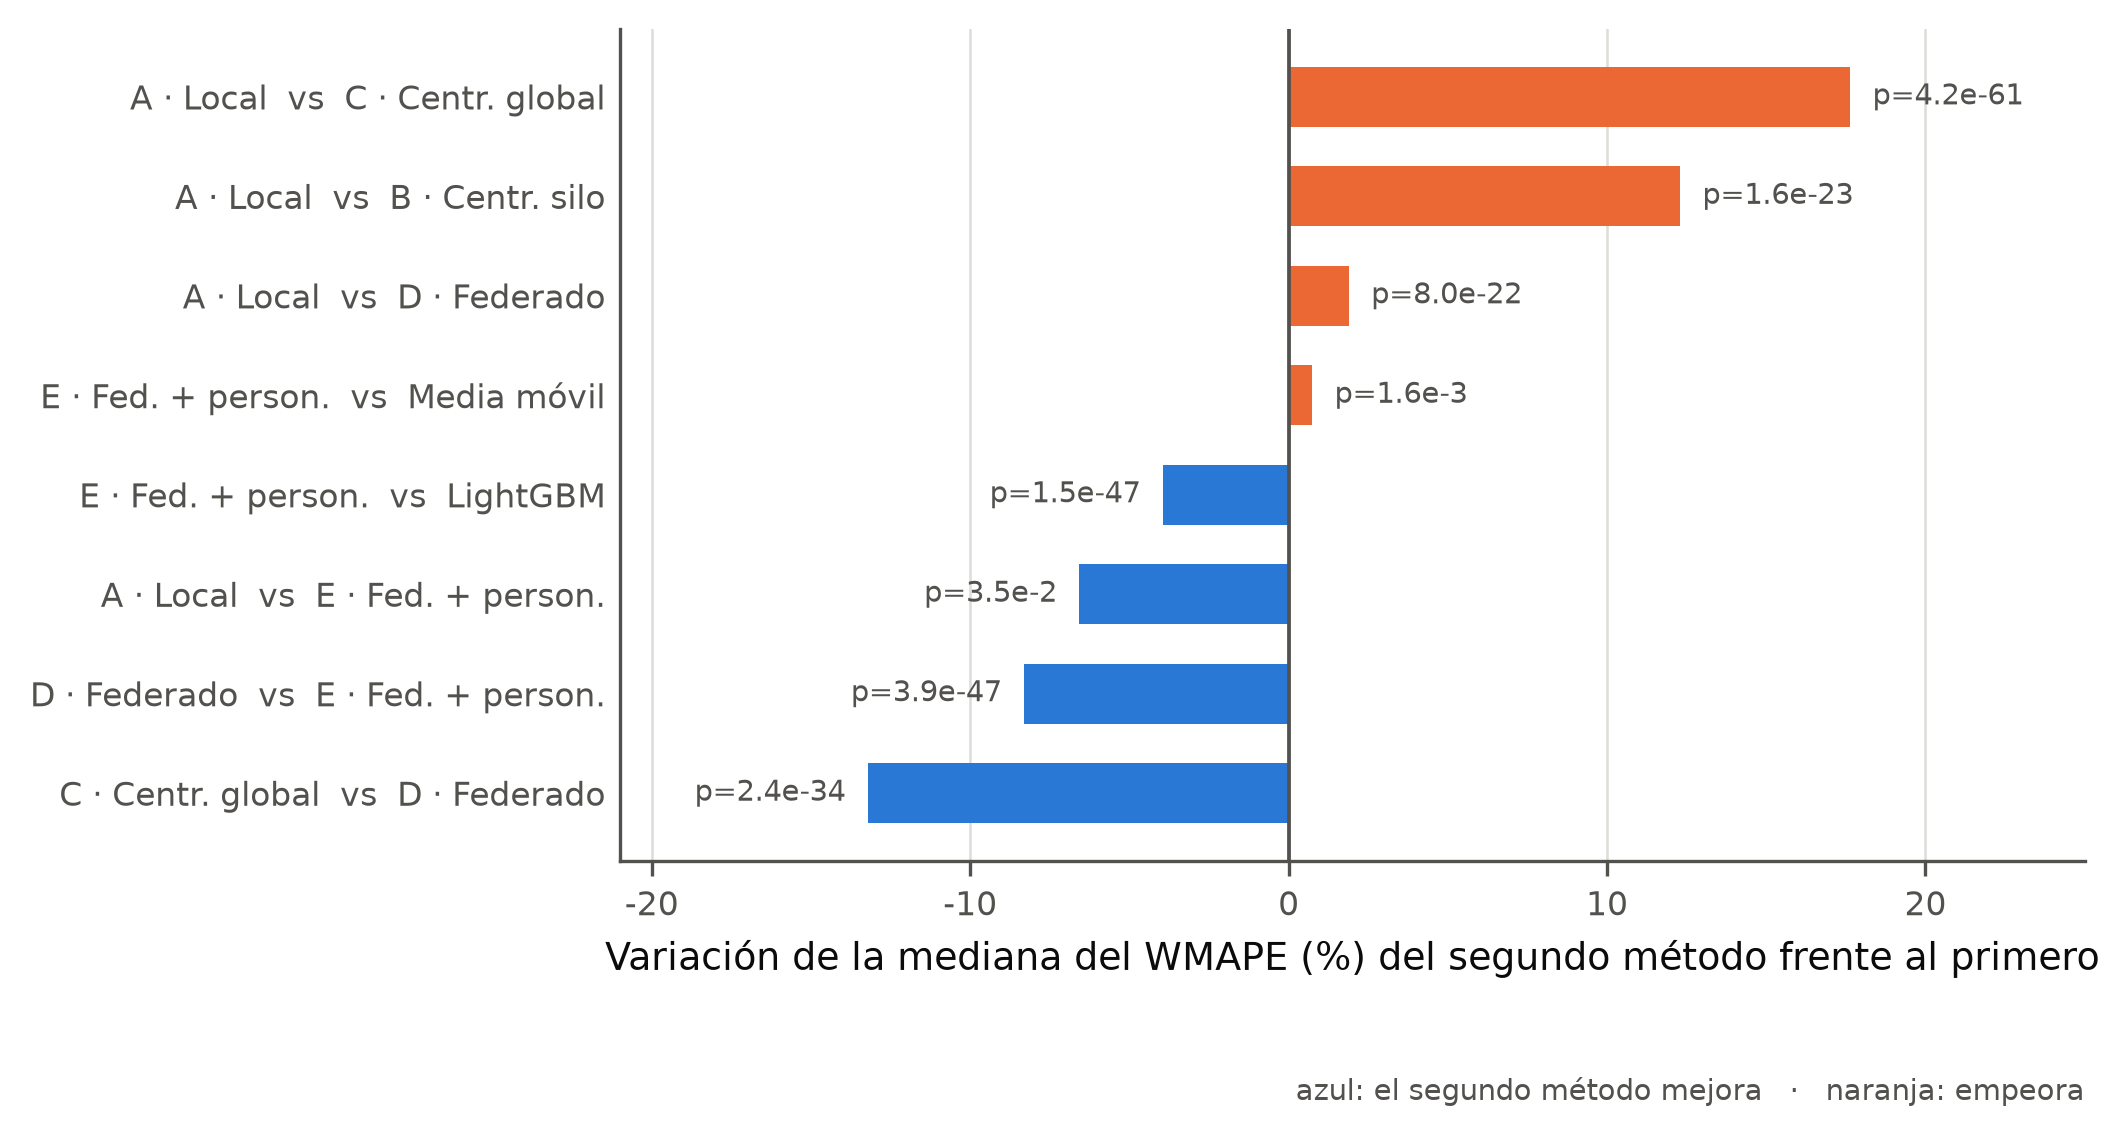
\includegraphics[width=\linewidth]{resultados_significancia.png}
\end{minipage}\hfill
\begin{minipage}[t]{0.43\linewidth}
\vspace{0pt}
{\fontsize{10.5}{13.5}\selectfont\color{grisTexto}%
Wilcoxon pareado por serie sobre las ocho comparaciones, con corrección de
Holm-Bonferroni. \textbf{Todos} resultan significativos al 5\,\%.\par}
\vspace{0.75em}

\bloque{tinta}{La escalera de centralización es real}{Que B y C sean peores que
  A son los dos contrastes con los p-valores más pequeños del estudio.}

\bloque{azul}{La personalización es la pieza que funciona}{D \emph{vs} E combina
  un efecto apreciable (--8,31\,\%) con significación muy alta.}

\bloque{naranja}{El valor de colaborar es real, pero es el efecto más débil}{El
  contraste A \emph{vs} E --- el que sostiene el análisis económico --- mejora un
  6,57\,\% con \emph{p} = 0,035: el menos robusto de los ocho.}

\pie{Sobre el aparente empate con la media móvil: las medianas globales se
  calculan sobre conjuntos de series distintos. En las 1.655 series comunes, E
  gana de forma significativa, pero solo por un 0,74\,\%.}
\end{minipage}

% ===========================================================================
% 11 — AZURE
% ===========================================================================
\diapo{5. Del simulador a la nube}{El esquema se comporta igual fuera de la simulación}

\begin{minipage}[t]{0.46\linewidth}
\vspace{0pt}
\cuerpo{Los resultados anteriores se obtuvieron con el motor de simulación de
  Flower, que representa los silos como procesos de una misma máquina. Eso no
  verifica que el esquema funcione sobre infraestructura realmente
  distribuida.}
\vspace{0.9em}

\bloque{aqua}{Tres máquinas virtuales independientes}{Cada una contiene
  \textbf{únicamente} el conjunto de datos de su silo. El aislamiento es
  efectivo, no simulado.}

\bloque{aqua}{El agregador se aloja en un silo}{Impuesto por la cuota de la
  suscripción, es un patrón legítimo en federaciones entre organizaciones y no
  altera el aislamiento: solo maneja parámetros.}

\pie{El despliegue exigió resolver restricciones de región, cuota de núcleos,
  consistencia eventual de los recursos y discrepancias de versión entre nodos.
  Todo quedó incorporado a los guiones de aprovisionamiento, de modo que el
  despliegue es reproducible.}
\end{minipage}\hfill
\begin{minipage}[t]{0.5\linewidth}
\vspace{0.5cm}
\centering
\begin{tikzpicture}[
    vm/.style={draw=regla,rounded corners=2pt,minimum width=3.1cm,
               minimum height=1.25cm,align=center,
               font=\footnotesize\color{tinta}},
    >={Stealth[round]}]
  \node[vm,fill=suave] (g) {\textbf{vm-silo-grande}\\{\scriptsize silo Grande + agregador}\\
    {\scriptsize solo \texttt{grande.parquet}}};
  \node[vm,below left=1.35cm and 0.35cm of g] (m) {\textbf{vm-silo-mediano}\\
    {\scriptsize solo \texttt{mediano.parquet}}};
  \node[vm,below right=1.35cm and 0.35cm of g] (p) {\textbf{vm-silo-pequeno}\\
    {\scriptsize solo \texttt{pequeno.parquet}}};
  \draw[<->,azul,line width=0.8pt] (g) -- node[sloped,above,font=\scriptsize\color{grisTexto}] {gRPC} (m);
  \draw[<->,azul,line width=0.8pt] (g) -- node[sloped,above,font=\scriptsize\color{grisTexto}] {gRPC} (p);
  \node[draw=regla,dashed,rounded corners=2pt,right=0.9cm of g,minimum width=2.4cm,
        minimum height=0.95cm,align=center,font=\footnotesize\color{tinta}] (aml)
    {Azure ML\\{\scriptsize métricas y registro}};
  \draw[->,grisTexto] (g) -- (aml);
  \begin{scope}[on background layer]
    \node[draw=regla,dashed,rounded corners=3pt,fit=(g)(m)(p),inner sep=0.3cm] (vnet) {};
  \end{scope}
  \node[font=\scriptsize\color{grisTexto},below=0.05cm of vnet] {red privada virtual};
\end{tikzpicture}
\end{minipage}

% ===========================================================================
% 12 — VALOR ECONÓMICO
% ===========================================================================
\diapo{6. Valor de negocio}{Cuánto vale colaborar en vez de entrenar en solitario}

\begin{minipage}[t]{0.30\linewidth}
\vspace{0pt}
\cifra{azul}{16,50\,\%}{menos error de previsión al pasar de A (local) a E
  (federado + personalización), \textbf{ponderando por volumen}}
\cifra{azul}{807.857}{unidades de error evitadas en las ocho semanas de prueba}
\cifra{aqua}{0,5 -- 3,9 M\texteuro}{ahorro anual estimado para la red de 54
  tiendas; escenario central 1,84 M\texteuro{}
  \mbox{($\approx$ 34.700 \texteuro/tienda)}}
\end{minipage}\hfill
\begin{minipage}[t]{0.31\linewidth}
\vspace{0pt}
\bloque{tinta}{Parte física y parte monetaria, separadas}{La reducción de error
  sale \emph{íntegramente} de los resultados del trabajo. La traducción a euros
  usa parámetros de sector y se presenta siempre como \textbf{rango con análisis
  de sensibilidad}, nunca como cifra única.}

\bloque{naranja}{El beneficio no es uniforme}{Se concentra en las series de
  mayor volumen --- las 50 primeras explican el \textbf{84,6\,\%} del ahorro ---
  y \textbf{764 de 1.655 series (46,2\,\%) empeoran}.}

\bloque{aqua}{Recomendación}{Seleccionar serie a serie, sobre validación, entre
  el modelo personalizado y el local.}
\end{minipage}\hfill
\begin{minipage}[t]{0.34\linewidth}
\vspace{0pt}
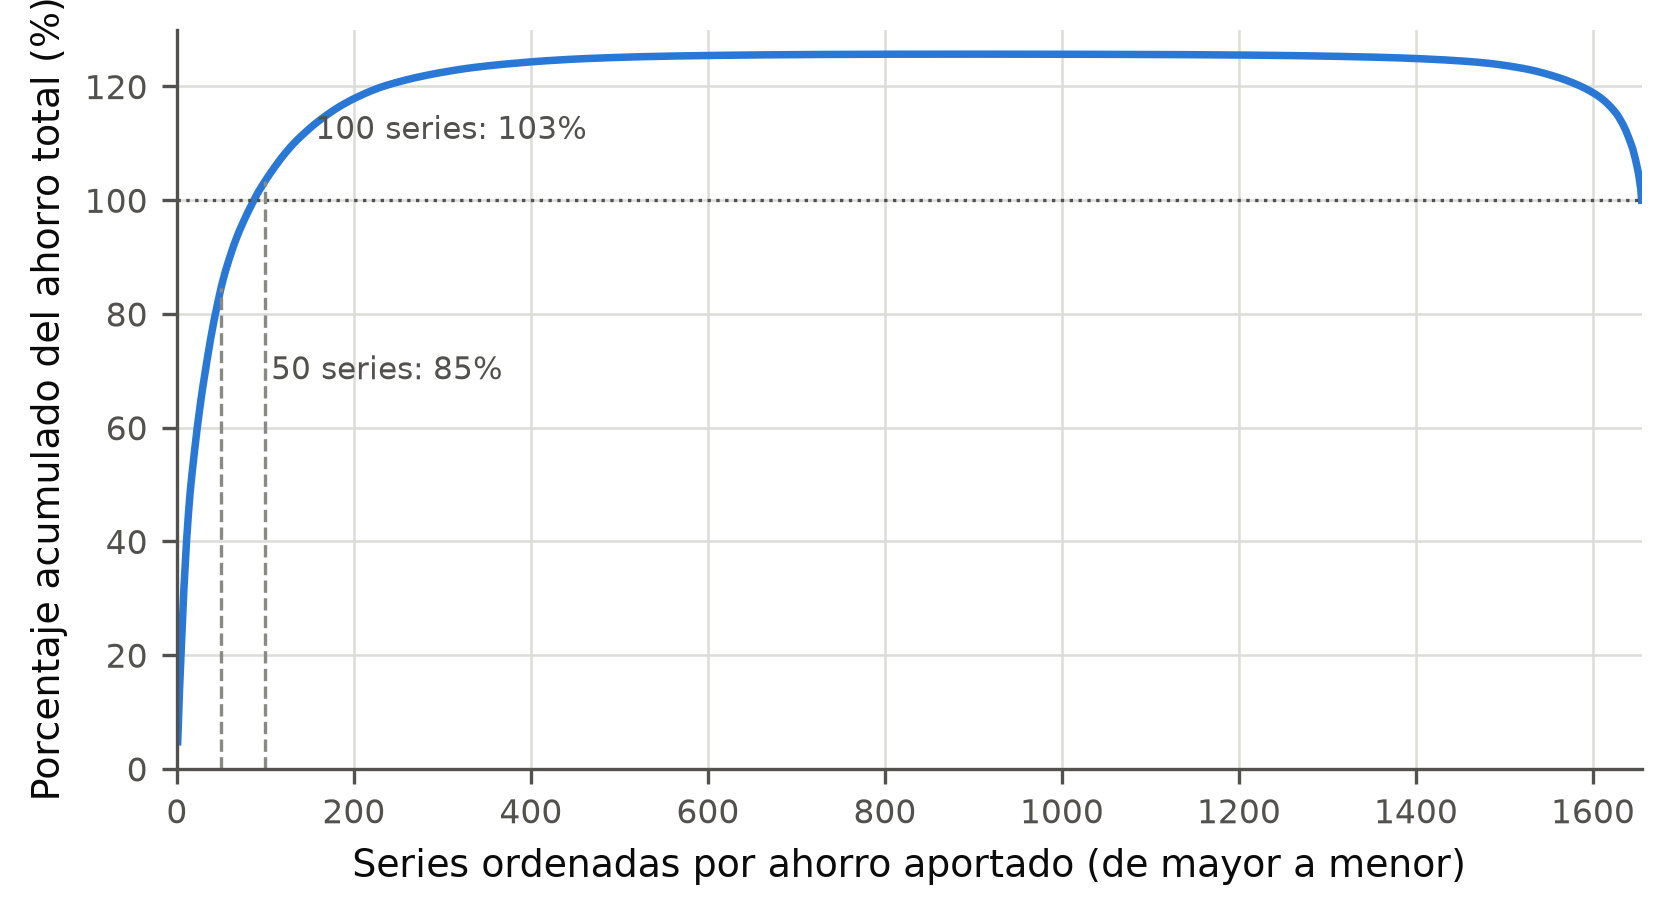
\includegraphics[width=\linewidth]{negocio_concentracion_ahorro.png}
\pie{La mediana de mejora es del 6,57\,\% y la ponderada por volumen del
  16,50\,\%: la personalización acierta justo donde hay volumen. Es la cifra
  económicamente relevante, pero también la que esconde a las series que
  empeoran.}
\end{minipage}

% ===========================================================================
% 13 — RQ4
% ===========================================================================
\diapo{6. Valor de negocio}{Por qué federado y no un \emph{data clean room}}

\begin{minipage}[t]{0.56\linewidth}
\vspace{0pt}
{\fontsize{10.5}{13.5}\selectfont
\begin{tabular}{@{}>{\raggedright\arraybackslash}p{2.4cm}%
                  >{\raggedright\arraybackslash}p{3.7cm}%
                  >{\raggedright\arraybackslash}p{3.7cm}@{}}
\toprule
{\color{tinta}\textbf{Dimensión}} &
{\color{tinta}\textbf{\emph{Data clean room}}} &
{\color{azul}\textbf{Aprendizaje federado}} \\
\midrule
{\color{grisTexto}Tarea que resuelve} &
{\color{grisTexto}Consultas sobre datos que ya existen} &
{\color{grisTexto}Entrenamiento de un modelo predictivo nuevo} \\
{\color{grisTexto}Movimiento de datos} &
{\color{grisTexto}Se copian a un entorno común} &
{\color{grisTexto}No salen de cada participante} \\
{\color{grisTexto}Tercero de confianza} &
{\color{grisTexto}Necesario: alguien opera el entorno} &
{\color{grisTexto}No custodia datos; solo parámetros} \\
{\color{grisTexto}Madurez} &
{\color{grisTexto}Alta, oferta comercial consolidada} &
{\color{grisTexto}Menor, marcos abiertos en evolución} \\
\bottomrule
\end{tabular}\par}
\end{minipage}\hfill
\begin{minipage}[t]{0.40\linewidth}
\vspace{0pt}
\bloque{azul}{La diferencia es de tarea, no de nivel de protección}{Un
  \emph{clean room} responde preguntas sobre datos que ya existen. Aquí hay que
  \textbf{construir} un modelo, lo que exigiría que todos depositaran sus datos
  crudos en el entorno de un tercero --- exactamente la cesión que se quería
  evitar.}

\bloque{tinta}{Y una consideración práctica}{Entre competidores, acordar
  \emph{quién} opera el entorno suele ser el verdadero obstáculo. El
  coordinador federado no custodia datos e incluso puede rotarse.}

\pie{\textbf{Matización necesaria:} no son alternativas excluyentes, sino
  primitivos distintos para problemas distintos. De hecho convergen. La
  conclusión se limita deliberadamente a esta tarea.}
\end{minipage}

% ===========================================================================
% 14 — CONCLUSIONES
% ===========================================================================
\diapo{7. Conclusiones}{Respuesta a las preguntas de investigación}

\begin{minipage}[t]{0.5\linewidth}
\vspace{0pt}
\bloque{azul}{RQ1 — Ninguna mitad coincide con la hipótesis}{El federado
  \emph{sin} personalizar no mejora al local. Y el centralizado no es el techo
  de rendimiento, sino el peor de los cinco. La afirmación correcta es más
  fuerte que la prevista: \textbf{E supera tanto al local como al
  centralizado}.}

\bloque{naranja}{RQ2 — Solo parcialmente}{Bate a persistencia, estacional y
  ETS; gana por poco a la media móvil; y \textbf{pierde} frente a LightGBM por
  un 3,95\,\% real.}

\bloque{aqua}{RQ3 — Valor real, con matices}{16,50\,\% menos error ponderado por
  volumen y del orden de 1,8 M\texteuro{} anuales, pero concentrado y con casi
  la mitad de las series empeorando.}

\bloque{aqua}{RQ4 — Resuelven tareas distintas}{Para \emph{entrenar} un modelo
  entre partes que no ceden datos, el federado es el primitivo adecuado.}
\end{minipage}\hfill
\begin{minipage}[t]{0.46\linewidth}
\vspace{0pt}
\colorbox{suave}{%
\begin{minipage}{\dimexpr\linewidth-1.6em}
\vspace{0.8em}
{\fontsize{12.5}{15}\selectfont\bfseries\color{tinta}Tres conclusiones de
alcance general\par}
\vspace{0.6em}
{\fontsize{11}{14.5}\selectfont\color{grisTexto}%
\textbf{1.} La personalización no es un añadido opcional al aprendizaje
federado, sino \textbf{la pieza que lo hace funcionar} en presencia de
heterogeneidad.\par\vspace{0.5em}
\textbf{2.} Más datos no implican mejor modelo \textbf{si la capacidad no
acompaña}. Que un LightGBM sí saque partido de esos mismos datos agregados
apunta al reparto de capacidad, no a la agregación.\par\vspace{0.5em}
\textbf{3.} Optimizar los hiperparámetros de una etapa aislada \textbf{puede
perjudicar a la siguiente}: el ajuste que mejoró D un 7\,\% empeoró la
personalización posterior.\par}
\vspace{0.9em}
\end{minipage}}

\vspace{0.7em}
\pie{RQ5 queda abierta y es la continuación más relevante: sin garantías
  formales, el esquema reduce la exposición pero no anonimiza.}
\end{minipage}

% ===========================================================================
% 15 — LÍNEAS FUTURAS Y CIERRE
% ===========================================================================
\diapo{7. Conclusiones}{Líneas futuras}

\begin{minipage}[t]{0.53\linewidth}
\vspace{0pt}
\begin{puntos}
  \item \textbf{\color{tinta}Privacidad diferencial y agregación segura}
    (RQ5), midiendo la curva de coste en precisión frente al presupuesto de
    privacidad. Es el paso necesario para poder sostener afirmaciones de
    anonimización.
  \item \textbf{\color{tinta}Selección por serie} entre modelo personalizado y
    local, decidida sobre validación: capturaría el beneficio de las series que
    mejoran evitando el perjuicio de las que empeoran.
  \item \textbf{\color{tinta}Ajuste de hiperparámetros específico} de la etapa
    de personalización, con una arquitectura más contenida.
  \item \textbf{\color{tinta}Validación con varios orígenes de previsión},
    desplazando la ventana temporal, para estimaciones más estables que las de
    un único corte de ocho semanas.
  \item \textbf{\color{tinta}Federación de modelos basados en árboles}, que en
    este problema son los más precisos y que no admiten el promediado de
    parámetros de FedAvg.
  \item \textbf{\color{tinta}Evaluación sobre operadores realmente distintos},
    que es la limitación de fondo del estudio.
\end{puntos}
\end{minipage}\hfill
\begin{minipage}[t]{0.42\linewidth}
\vspace{1.2cm}
{\color{azul}\rule{3.2cm}{2.5pt}}\par\vspace{1.0em}
{\fontsize{15}{19}\selectfont\bfseries\color{tinta}%
El detalle completo está en la memoria\par}
\vspace{0.7em}
{\fontsize{11}{14.5}\selectfont\color{grisTexto}%
59 páginas, 8 capítulos y anexos, con la metodología, los resultados
intermedios, la discusión y las limitaciones desarrolladas.\par
\vspace{0.7em}
Todo el código, los resultados y el cuaderno de laboratorio del proyecto están
versionados en el repositorio.\par}
\vspace{1.4em}
{\fontsize{12}{15}\selectfont\bfseries\color{tinta}Alessandro Flammia\par}
{\fontsize{10.5}{13}\selectfont\color{grisTexto}Máster en Análisis de Datos en
Ingeniería --- Tecnun\par}
\end{minipage}

\end{document}
